\documentclass[a4paper,12pt, english]{article}
\usepackage[T1]{fontenc}
\usepackage[utf8]{inputenc}
\usepackage{graphicx}
\usepackage{babel}
\usepackage{amsmath}
\usepackage{ulem}
\usepackage{a4wide}
\usepackage{graphicx}
\usepackage{listings}
\usepackage{tabularx}
\usepackage{tabulary}
\usepackage{hyperref}

\begin{document}

\begin{titlepage}
\begin{center}
\textsc{\Large Machine Learning}\\[0.2cm]
\textsc{FYS-STK 4155}\\[1.0cm]
\textsc{\Large Project 1}\\[0.2cm]
\textsc{Kari Eriksen}\\[1.0cm]

\begin{abstract}
Here is my abstract going to be
\end{abstract}

\end{center}
\end{titlepage}

\section*{Introduction}

One of the simples models within the field of machine learning and statistical learning is linear regression. Because of its simplicity and the fact that it forms the base of many other more advanced methods it is highly recommended to understand it. \\ 
In this project we are studying several linear regression methods, the ordinary least square, Ridge regression and last the Lasso regression. Our first approach to understand these methods is to test them on the Franke function \ref{eq:frank}, a two-dimensional function which is widely used on testing interpolation and fitting algorithms. 
We evaluate our models abillity to predict the outcome(solution) using a resampling method called bootstrap and explore statistical errors such as bias, variance and Mean Square Error (MSE). All methods are explained in the sections below. \\
At last we will be using real data from a website that provides terrain data over the earth, \href{https://earthexplorer.usgs.gov/}{https://earthexplorer.usgs.gov/}, and test out method on these. 

 

\section*{Theory}

\begin{figure}
\centering
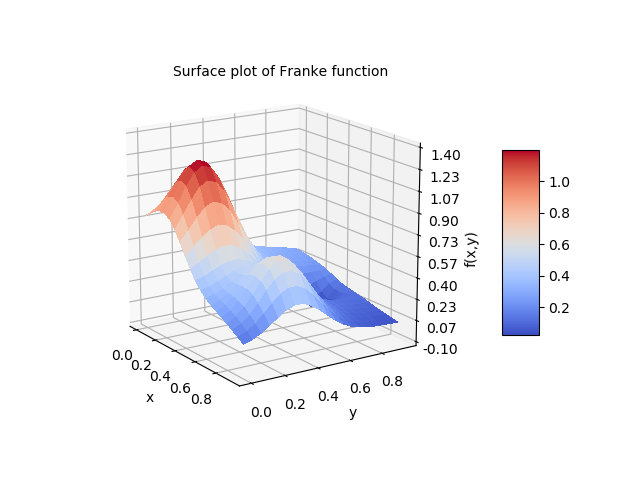
\includegraphics[width=1.0\textwidth]{/home/kari/Machine-Learning/Figures/franke.png}
\caption{Surface plot of Franke function for $x, y \in [0,1]$ generated with python code given in the assigment paper.}
\label{fig:franke}
\end{figure}


The Franke function is a two-dimensional function consisting of a sum of four exponatials, eq. \ref{eq:frank}. This will be the function which we will generate data from to feed our regression models. We define it for $x, y \in [0,1]$. \\
It can be seen represented as a surface plot in figure \ref{fig:franke}.

\begin{align}
f(x,y) &= \frac{3}{4}\exp{\left(-\frac{(9x-2)^2}{4} - \frac{(9y-2)^2}{4}\right)}+\frac{3}{4}\exp{\left(-\frac{(9x+1)^2}{49}- \frac{(9y+1)}{10}\right)} \nonumber \\
&+\frac{1}{2}\exp{\left(-\frac{(9x-7)^2}{4} - \frac{(9y-3)^2}{4}\right)} -\frac{1}{5}\exp{\left(-(9x-4)^2 - (9y-7)^2\right) } \label{eq:frank}
\end{align}




\section*{Regression methods}

\subsection*{Linear Regression}

Linear regression is a method in statistics that predicts the response of one or several explanatory variables. At its simplest form we could try to find the stright line between two points. This equation is fairly simple.

\begin{equation}
\hat{y} = \hat{\beta_{0}} + \hat{\beta_{1}}x + \epsilon
\end{equation}

Here $\hat{y}$ is a dependent variable, the outcome, $x$ is an independent variable, or the predictor, and $\hat{\beta_{0}}$ and $\hat{\beta_{1}}$ the intercept and slope respectively. $\epsilon$ is the error in our prediction. \\
If we had several predictors we could extend our problem to a more general case.

\begin{equation}
\hat{y} = f(X) = \beta_{0} + \sum_{j=1}^{p} X_{j} \beta_{j}
\end{equation}

Now $X$ is a vector containing all predictors, $X^{\top} = \{X_0, X_1, X_2, X_3,..., X_p\}$, $\beta_0$ is the intercept and $\beta_j$ is a vector keeping all coefficients for each predictor, the parameters we are searching for. Moving $\beta_0$ to the $\beta-\textnormal{vector}$ and adding an extra column with 1's to the design matrix $X^{\top}$ we can reduce the problem to vector form and get the following.


\begin{equation}
\hat{y} = \hat{X} \hat{\beta} + \epsilon
\end{equation}

\begin{equation}
y_i = \beta_0 + \beta_1 x_i + \beta_2 x_i^{2} + \beta_3 x_i^{3} + \beta_4 x_i^{4} + ... + \beta_d x_i^{d}
\end{equation}


\subsection*{Ordinary Least Square}

\begin{equation}
\textnormal{RSS}(\beta) = \sum_{i=1}^{N} (y_i - x_i^{\top}\beta)^2
\end{equation}

\begin{equation}
\textnormal{RSS}(\beta) = (\mathbf{y} - \mathbf{X}\beta)^{\top}(\mathbf{y} - \mathbf{X}\beta)
\end{equation}

\begin{equation}
\frac{\partial \textnormal{RSS}(\beta)}{\partial \beta} = 0 = -2 \mathbf{X}^{\top}(\mathbf{y} - \mathbf{X}\beta)
\end{equation}

\begin{equation}
\mathbf{X}^{\top}\mathbf{y} - \mathbf{X}^{\top}\mathbf{X} \beta = 0
\end{equation}

\begin{equation}
\hat{\beta} = (\mathbf{X}^{\top}\mathbf{X})^{-1}\mathbf{X}^{\top}\mathbf{y}
\end{equation}

\subsection*{Ridge Regression}

\begin{equation}
\hat{y} = \hat{X} \hat{\beta} + \epsilon
\end{equation}

\begin{equation}
\hat{\beta} = (\mathbf{X}^{\top}\mathbf{X} + \lambda\mathbf{I}_{pp})^{-1}\mathbf{X}^{\top}\mathbf{Y}
\end{equation}

\subsection*{Lasso Regression}


\section*{Resampling method}



\subsection*{Bootstrap}

Evaluate some statistical estimates

\section*{Results}

Hope I get some results...

\section*{Discussion}

..to discuss. 

\end{document}